\section{Auswertung}

\subsection*{Vorbemerkungen}

Sofern nicht anders angegeben, berechnen wir die Fehler zusammengesetzter Werte anhand der standardmäßigen Gauß'schen Fehlerfortpflanzung. Die $\sigma$-Abweichung zweier fehlerbehafteter Werte $x \pm \Delta x$ und $y \pm \Delta y$ berechnen wir anhand der Formel
\begin{align}
  \sigma = \frac{\qty|x - y|}{\sqrt{\Delta x^2 + \Delta y^2}}.
\end{align}

Für eine Anzahl an Ereignissen $N$ berechnet sich der Fehler gemäß $\Delta N = \sqrt{N}$. Zur Fehlerangabe für Zählraten $n = \flatfrac{N}{t}$ leiten wir daraus die Formel
\begin{align}
  \Delta n = \frac{\Delta N}{t}= \frac{\sqrt{N}}{t} = \frac{\sqrt{nt}}{t} = \sqrt{\frac{n}{t}}
\end{align}
ab.

\subsection{Röntgenspektrum mit LiF-Kristall}

\abbref{fig:spektrum_lif_komplett} zeigt das Röntgenspektrums, welches wir mit der Drehkristallmethode mit einem LiF-Kristall im Winkelbereich von $3\si{\degree}$ bis $22\si{\degree}$ aufgezeichnet haben. Bereits hier ist zu erkennen, dass wir ab einem Winkel von etwa $5\si{\degree}$ beginnen, Bremsstrahlung zu detektieren.

\begin{figure}[H]
  \centering
  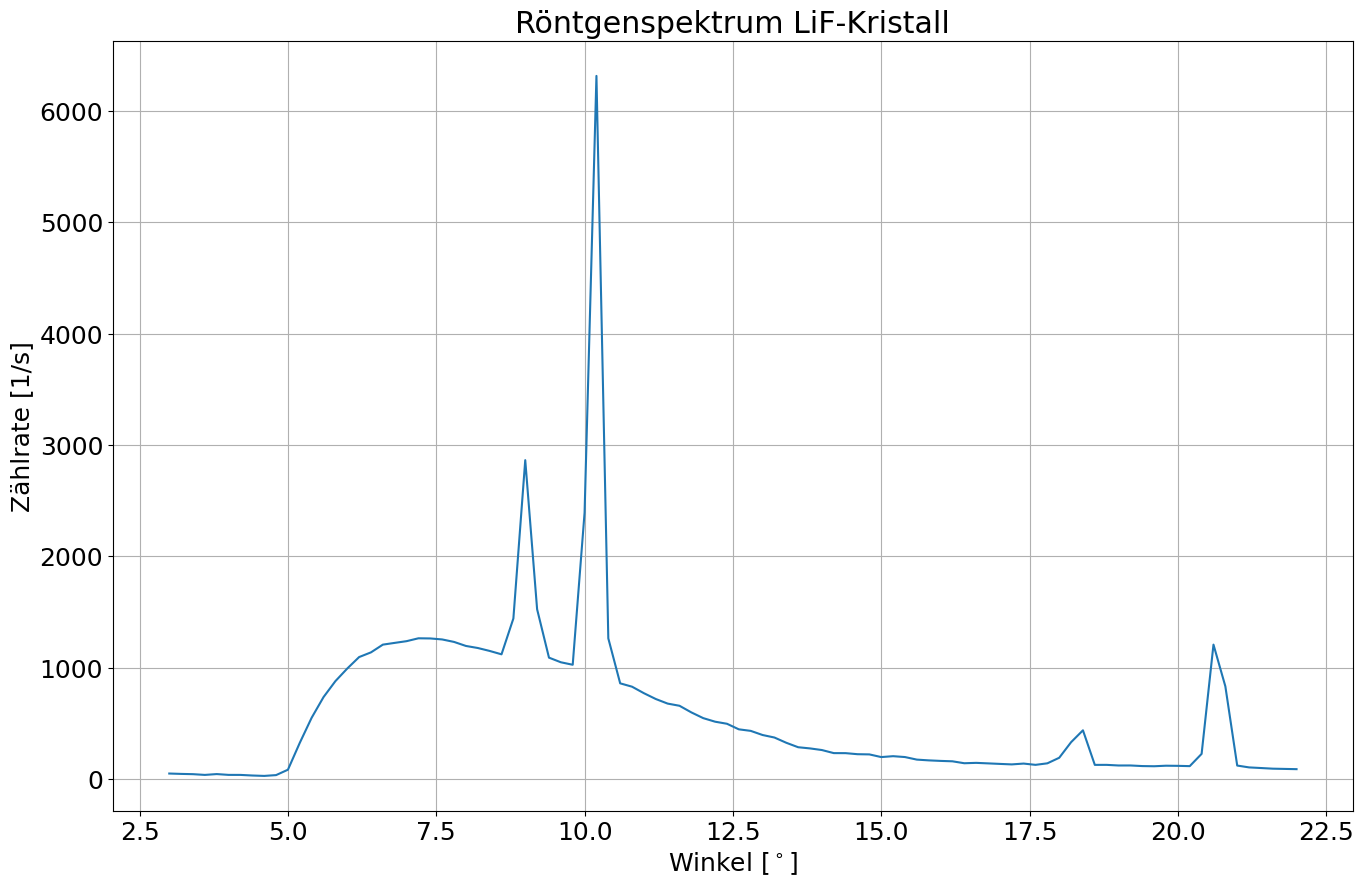
\includegraphics[width=.9\textwidth]{files/plots/spektrum_lif_komplett.png}
  \caption{Röntgenspektrum, ausgemessen mit LiF-Kristall.}
  \label{fig:spektrum_lif_komplett}
\end{figure}

Um den Winkel und die zugehörige Grenzwellenlänge genauer zu bestimmen, betrachten wir den nahezu linearen Bereich des Spektrums am kurzwelligen Ende und fitten an dieses eine lineare Funktion der Form $f(x;a,b) = ax + b$, wie in \abbref{fig:spektrum_lif_linear_fit} zu sehen.

\begin{figure}[H]
  \centering
  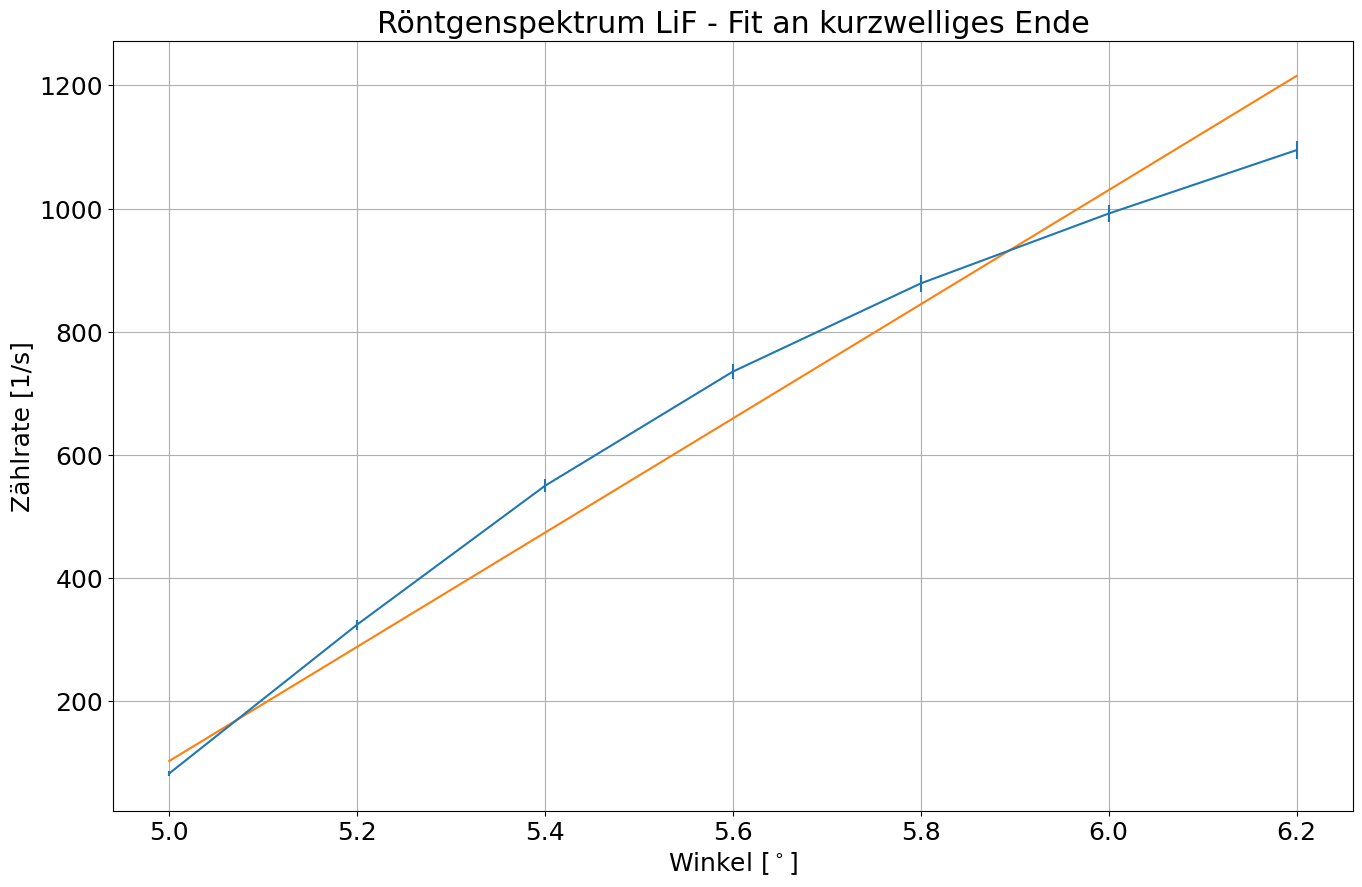
\includegraphics[width=.9\textwidth]{files/plots/spektrum_lif_linear_fit.png}
  \caption{Linearer Fit an das kurzwellige Ende des zuvor gezeigten Röntgengenspektrums.}
  \label{fig:spektrum_lif_linear_fit}
\end{figure}

Für die optimierten Parameter erhalten wir die Werte
\begin{align}
  a = 926.94 \pm 56.62 \si{\per\second\per\degree},\quad
  b = -4531.53 \pm 297.50 \si{\per\second}.
\end{align}
Mit diesen berechnen wir den Winkel, ab dem die Bremsstrahlung einsetzt, als Nullstelle der linearen Funktion nach
\begin{align}
  \vartheta_{0,1. Ord} = -\frac{b}{a} = 4.9 \pm 0.5 \si{\degree}.
\end{align}

Mithilfe des Bragg'schen Gesetzes \eqref{eq:bragg} können wir daraus nach
\begin{align}
  \lambda = \frac{2d\sin(\vartheta)}{n}
\end{align}
die entsprechende Grenzwellenlänge berechnen. Da es sich hierbei um den Einsatz des Spektrums erster Ordnung handelt, setzen wir $n = 1$. Den Netzebenenabstand $d$ des LiF-Kristalls entnehmen wir aus der Praktikumsanleitung als $d = 201.4\si{\pico\meter}$. Damit erhalten wir für die Grenzwellenlänge einen Wert von
\begin{align}
  \lambda_{Grenz} = (34.33 \pm 3.08) \si{\pico\meter}.
\end{align}

Setzen wir nun in \eqref{eq:grenzfreq} diese Grenzwellenlänge, die Spannung $U = 35\si{\kilo\volt}$ ein und stellen diese nach dem Plank'schen Wirkungsquantum $h$ um, so erhalten wir für dieses einen Wert von
\begin{align}
  h = (6.4 \pm 0.6) \cdot 10^{-34} \si{\joule\second}.
\end{align}

Die Grenzwellenlänge $\lambda_{grenz}$ können wir weitergehend einsetzen, um den Winkel zu bestimmen, ab dem das Spektrum zweiter Ordnung einsetzt. Dazu stellen wir \eqref{eq:bragg} nach $\vartheta$ um, und setzen $n = 2$. Wir erhalten damit einen Winkel von
\begin{align}
  \vartheta_{0,2. Ord} = (9.813 \pm 0.016)\si{\degree}.
\end{align}

\subsection{Bestimmung der Wellenlängen der $K_{\alpha,\beta}$-Linien}

Wir betrachten nun die Wellenlängenbereiche, in welchen die $K_{\alpha}$- und $K_{\beta}$-Linien erster und zweiter Ordnung zu sehen sind, genauer. Die Ausschnitte, aufgenommen in Winkelschritten von $0.1\si{\degree}$, sind in \abbref{fig:lif_kalpha_kbeta} zu sehen.

\begin{figure}[H]
  \centering
  \begin{minipage}{0.5\textwidth}
      \centering
      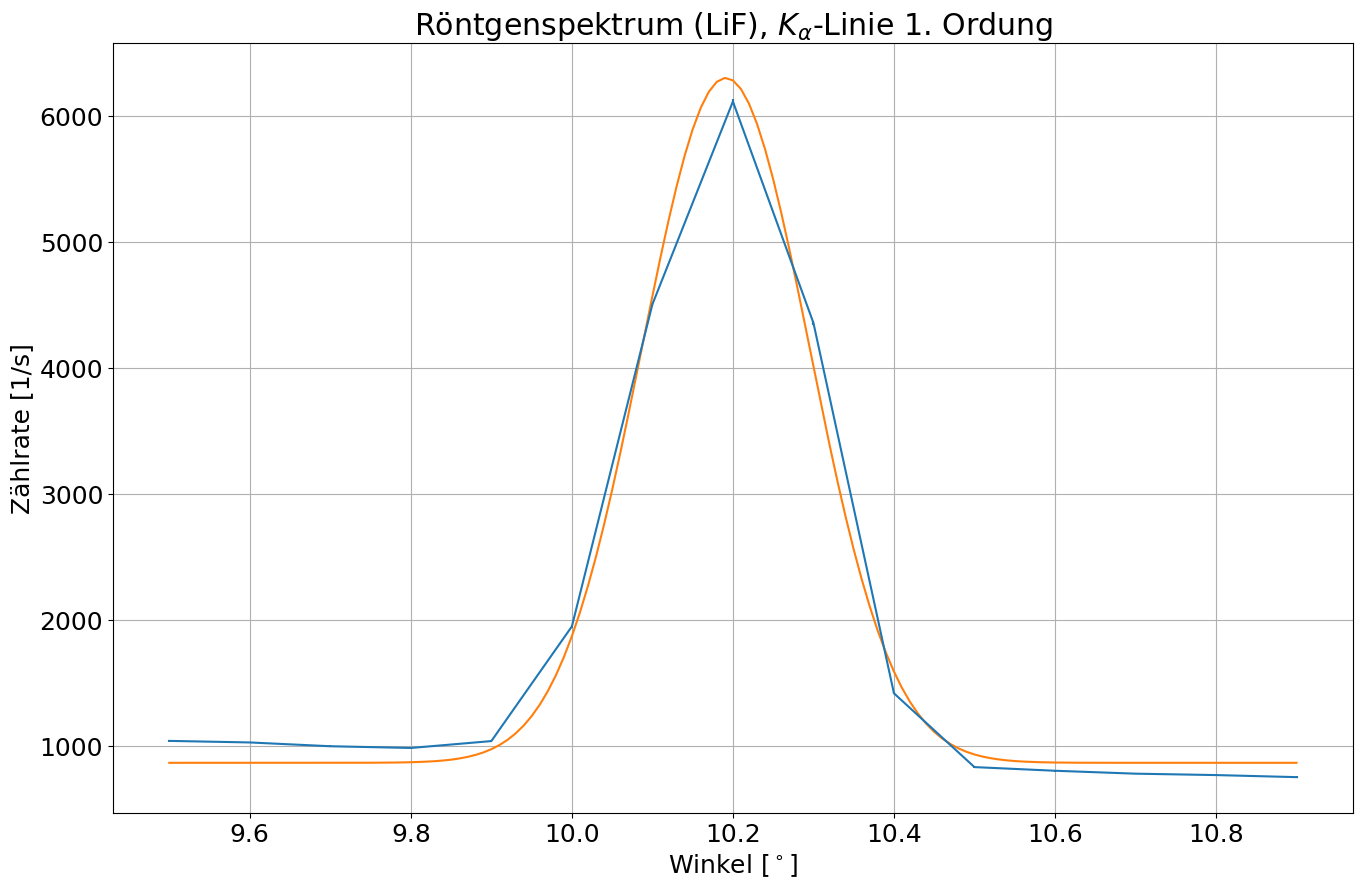
\includegraphics[width=0.99\textwidth]{files/plots/lif_kalpha_1ord.png}
  \end{minipage}\hfill
  \begin{minipage}{0.5\textwidth}
      \centering
      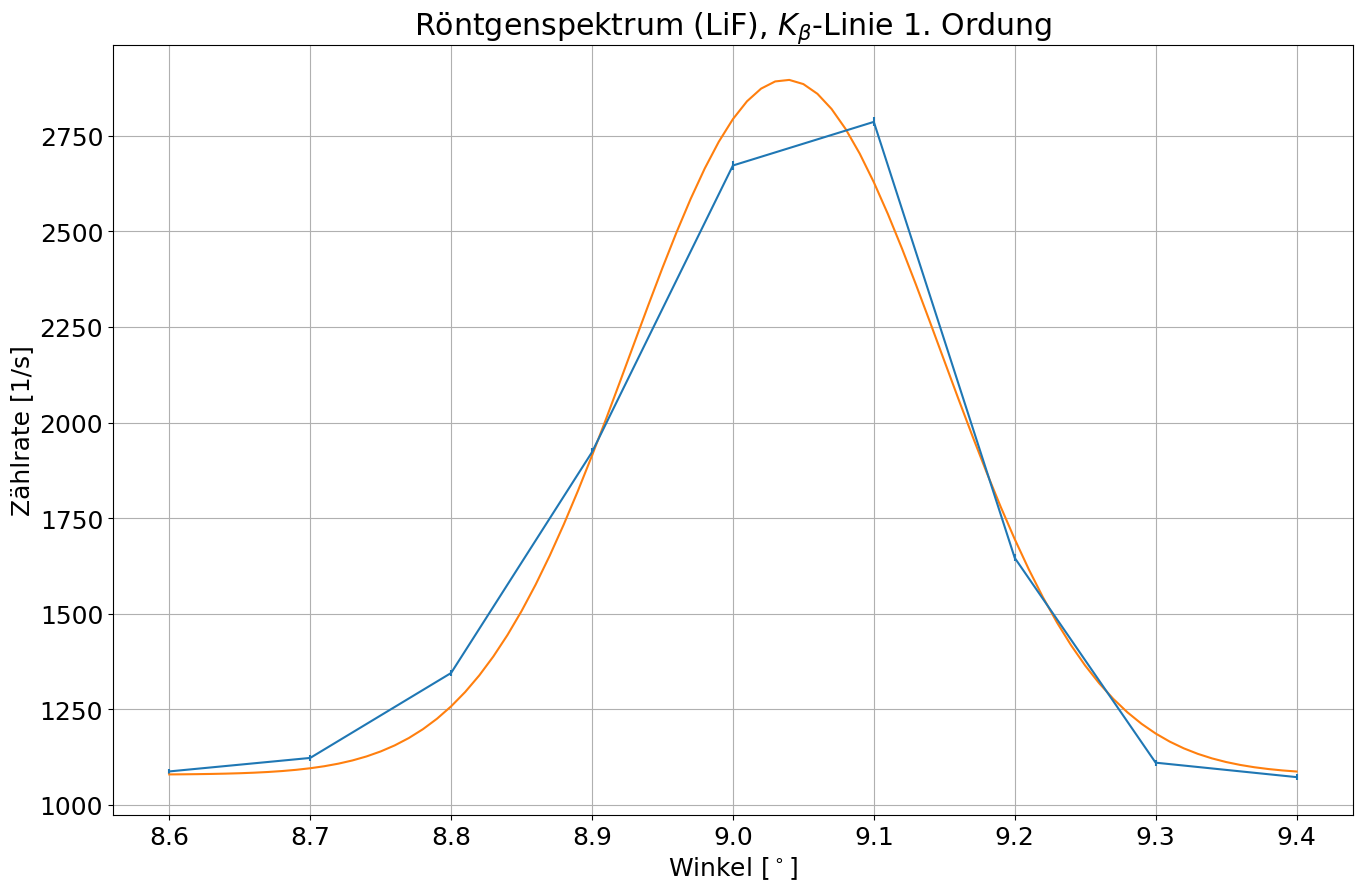
\includegraphics[width=0.99\textwidth]{files/plots/lif_kbeta_1ord.png}
  \end{minipage}\\
  \begin{minipage}{0.5\textwidth}
    \centering
    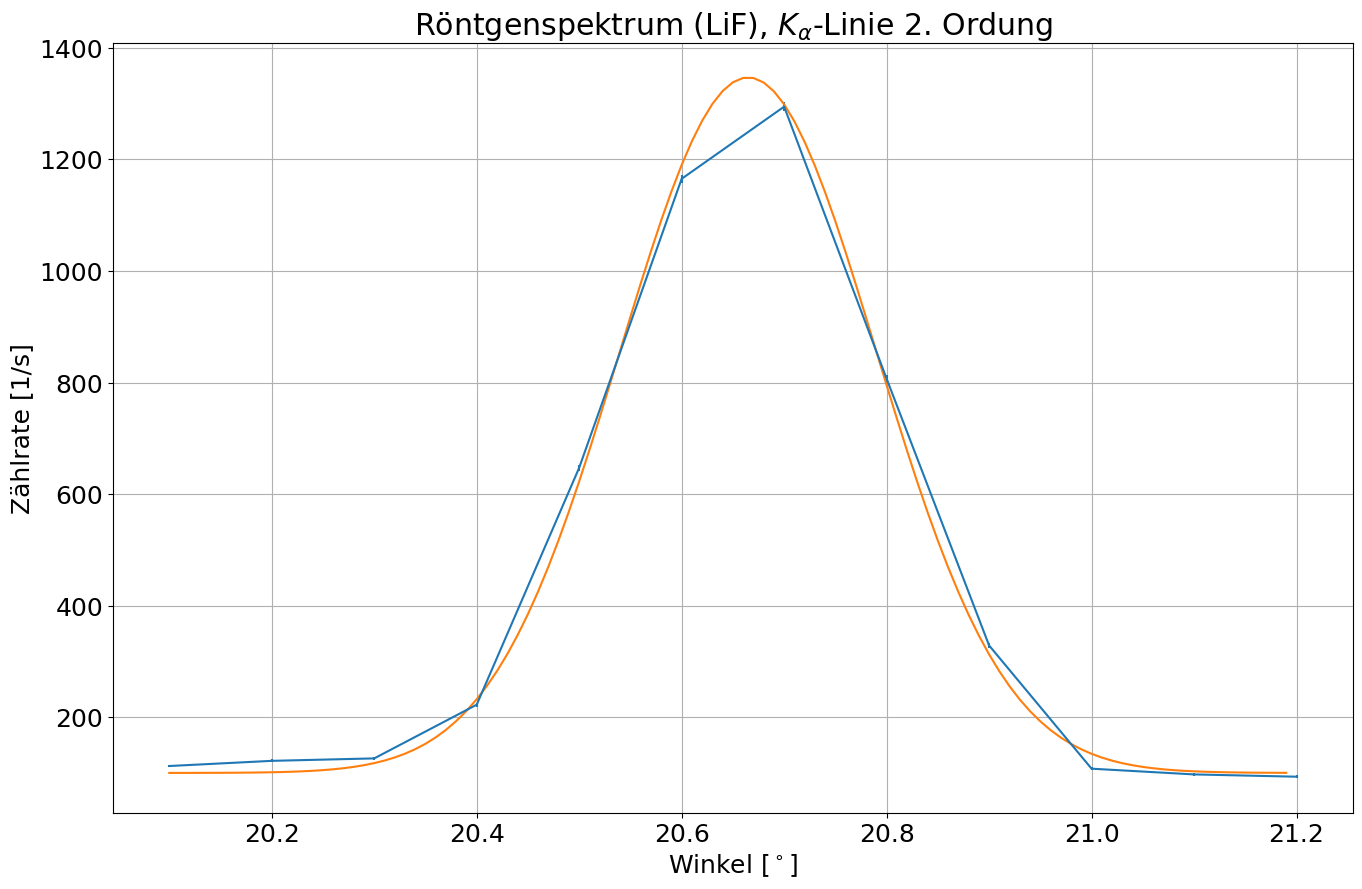
\includegraphics[width=0.99\textwidth]{files/plots/lif_kalpha_2ord.png}
\end{minipage}\hfill
\begin{minipage}{0.5\textwidth}
    \centering
    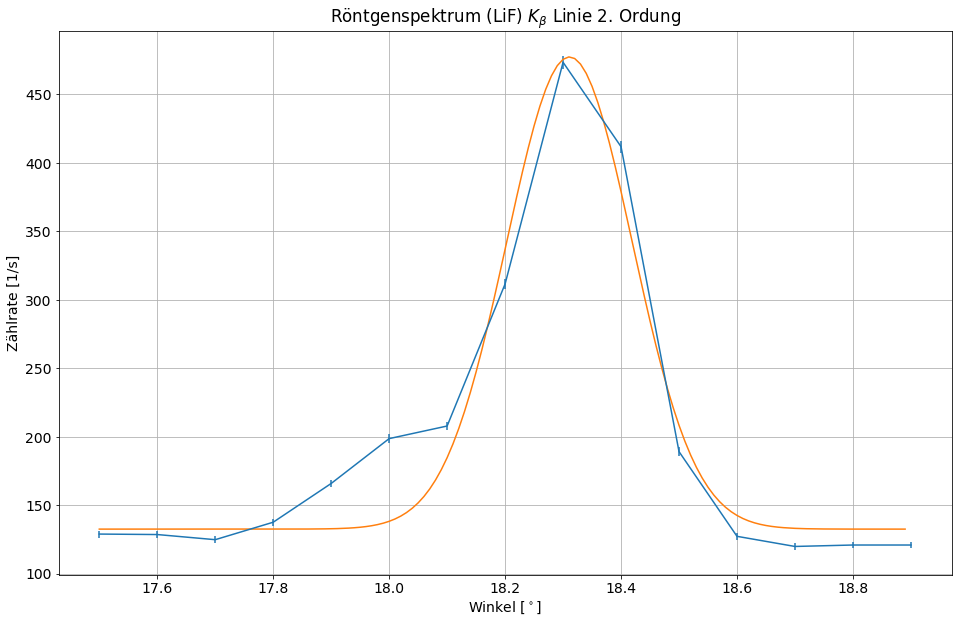
\includegraphics[width=0.99\textwidth]{files/plots/lif_kbeta_2ord.png}
\end{minipage}
\caption{$K_{\alpha}$- und $K_{\beta}$-Linien erster Ordnung (oben) und zweiter Ordnung (unten).}
\label{fig:lif_kalpha_kbeta}
\end{figure}

Um die Lage der Linien, sowie die Halbwertsbreite, zu ermitteln, fitten wir an die Daten eine Exponentialfunktion der Form
\begin{align}
  f(x;A,\mu,\sigma,c) = \frac{A}{\sqrt{2 \pi}\sigma} \exp(\frac{-(x - \mu)^2}{2 \sigma^2}) + c.
\end{align}
Die Halbwertsbreite ermitteln wir dann aus der Standardabweichung $\sigma$ nach der Formel
\begin{align}
  \fwhm = 2\sqrt{2\ln(2)}\sigma.
\end{align}

Der optimierte Wert von $\mu$ beschreibt hier erneut den \textit{Winkel} des Kristalls, bei welchem sich die Linie befindet. Um daraus die zugehörigen Wellenlängen zu berechnen, verwenden wir wieder das Bragg'sche Gesetz \eqref{eq:bragg}, mit entsprechendem $n \in \qty{1,2}$ für die Linien erster bzw. zweiter Ordnung. Bei der Berechnung der Wellenlänge verwenden wir den Wert $\flatfrac{\sigma}{\sqrt{N}}$ als Fehler des Winkels. Hierbei ist $\sigma$ die Standardabweichung der optimierten Gaußkurve und $N$ die Länge des Datensatzes, auf dem der Fit durchgeführt wurde. Die Ergebnisse sind in \tabref{tab:lif_k_alpha_beta} zusammengefasst.

\begin{table}[H]
  \centering
  \caption{Ergebnisse des Röntgenspektrums (LiF) für die $K_{\alpha}$- und $K_{\beta}$-Linien in der 1. und 2. Ordnung.}
  \vspace*{0.5em}
  \begin{tabular}{c|c|c|c|c||c}
    Linie & Ordnung & Mittelw. $\qty[\si{\degree}]$ & Stabw. $\qty[\si{\degree}]$ & FWHM $\qty[\si{\degree}]$ & $\lambda$ $\qty[\si{\pico\meter}]$\\\hline
    $K_{\alpha}$ & 1 & $10.191 \pm 0.005$ & $0.104 \pm 0.005$ & $0.245 \pm 0.011$ & $71.27 \pm 0.19$ \\
    $K_{\beta}$  & 1 & $9.038 \pm 0.007$  & $0.110 \pm 0.008$ & $0.260 \pm 0.018$ & $63.27 \pm 0.26$ \\\hline
    $K_{\alpha}$ & 2 & $20.665 \pm 0.004$ & $0.125 \pm 0.004$ & $0.294 \pm 0.008$ & $71.07 \pm 0.12$ \\
    $K_{\beta}$  & 2 & $18.311 \pm 0.011$ & $0.109 \pm 0.011$ & $0.256 \pm 0.025$ & $63.27 \pm 0.10$ \\\hline
  \end{tabular}
  \label{tab:lif_k_alpha_beta}
\end{table}

Aus den Werten der Wellenlängen der Linien erster und zweiter Ordnung bilden wir nun noch die Mittelwerte, um mit diesen später weiterzurechnen:
\begin{align}
  \lambda_{K_{\alpha}} = (71.17 \pm 0.12)\si{\pico\meter},\label{res:wl_kalp}\\[1em]
  \lambda_{K_{\beta}} = (63.27 \pm 0.14)\si{\pico\meter}.\label{res:wl_kbet}
\end{align}

Diese beiden Werte sind charakteristisch für die Molybdänanode der Röntgenröhre.

\subsection{Zählrate als Funktion der Beschleunigungsspannung}

Bei einem festen Winkel des LiF-Kristalls von $7.5\si{\degree}$ haben wir die Zählraten für die Beschleunigungsspannungen im Bereich von $20$ bis $35\si{\kilo\volt}$ aufgezeichnet. Die Daten sind in \abbref{fig:lif_ang75_volt_fit} zu sehen.

\begin{figure}[H]
  \centering
  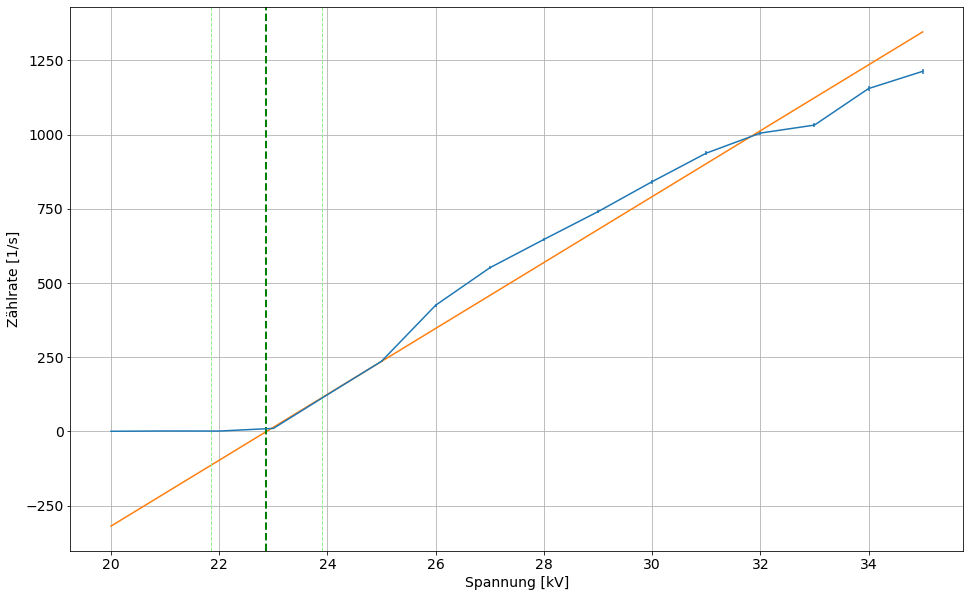
\includegraphics[width=.9\textwidth]{files/plots/lif_ang75_volt_fit.png}
  \caption{Zählraten bei steigender Beschleunigungsspannung unter einem Winkel von $7.5\si{\degree}$.}
  \label{fig:lif_ang75_volt_fit}
\end{figure}

Ebenfalls in \abbref{fig:lif_ang75_volt_fit} zu sehen ist eine linearer Funktion, welchen wir an diese Daten angepasst haben, um die Nullstelle, also den Punkt, ab dem die Aussendung von Bremsstrahlung einsetzt, zu finden. Nach dem gleichen Schema wie zuvor, können wir anhand der optimierten Parameter der linearen Funktion deren Nullstelle zu einem Wert von
\begin{align}
  U_0 = (22.9 \pm 1.1)\si{\kilo\volt}
\end{align}
bestimmen. Die zu einem Winkel von $7.5\si{\degree}$ korrespondierende Wellenlänge berechnen wir auf
\begin{align}
  \lambda_{7.5} = (52.6 \pm 0.4)\si{\pico\meter}.
\end{align}

Die ermittelte Wellenlänge und die Einsatzspannung können wir nun erneut in Gleichung \eqref{eq:grenzfreq} einsetzen, um das Planck'sche Wirkungsquantum zu bestimmen. Hier erhalten wir einen Wert von
\begin{align}
  h = (6.43 \pm 0.30) \cdot 10^{-34}
\end{align}

\subsection{Röntgenspektrum, ausgemessen mit NaCl-Kristall.}

Wir haben die Messung aus Versuchsteil 1 wiederholt und die Drehkristallmethode mit einem NaCl-Kristall angewandt, um das Röntgengenspektrum in einem Winkelbereich von $3\si{\degree}$ bis $18\si{\degree}$ aufzuzeichnen. Dieses ist in Gänze in \abbref{fig:spektrum_nacl_komplett} zu sehen.

\begin{figure}[H]
  \centering
  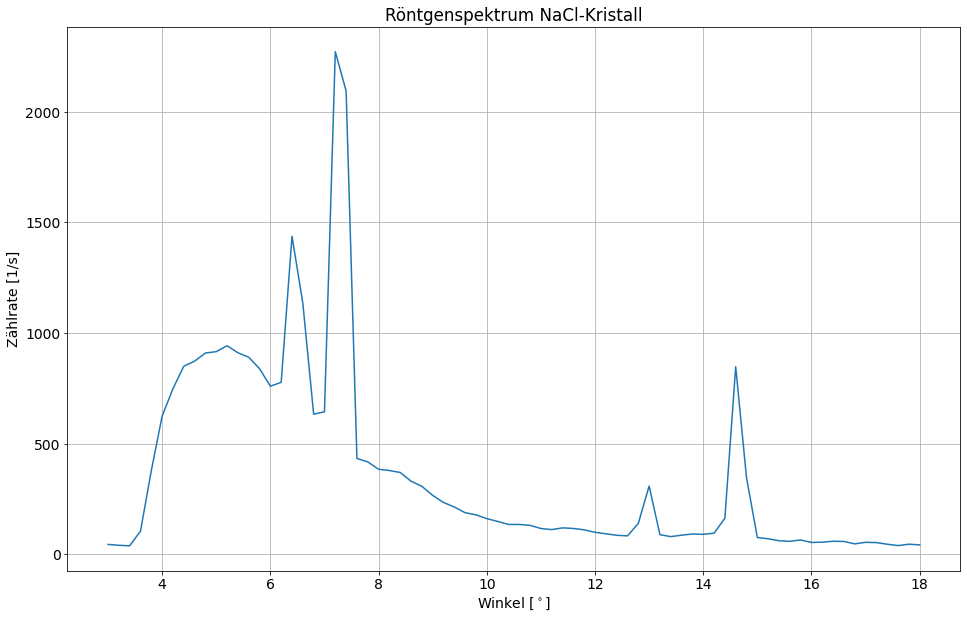
\includegraphics[width=.9\textwidth]{files/plots/spektrum_nacl_komplett.png}
  \caption{Röntgenspektrum mit NaCl-Kristall.}
  \label{fig:spektrum_nacl_komplett}
\end{figure}

Ziel ist es in diesem Aufgabenteil, die Gitterkonstante von NaCl zu ermitteln. Wir wissen, dass diese gerade dem Doppelten des Netzebenenabstands $d$ entspricht, welchen wir über das Bragg'sche Gesetz 
\begin{align}
  d = \frac{n \lambda}{2 \sin(\vartheta)}\label{eq:d_by_bragg}
\end{align}
ermitteln können.

Hierzu ermitteln wir nun erneut die Winkelpositionen der $K_{\alpha}$- und $K_{\beta}$-Linien erster Ordnung, um diese mit den Wellenlängen der Linien aus Aufgabe 2 zu identifizieren. Dies können wir tun, da diese Werte charakteristisch für die Molybdänanode der Röntgenröhre sind und damit unabhängig von der Art des Kristalls. Mit einem Fit zweier Gaußkurven an die beiden Linien erster Ordnung, zu sehen in \abbref{fig:nacl_k_1ord_fit}, ermitteln wir die Winkel zu
\begin{align}
  \beta_{K_{\alpha}} = 7.30 \pm 0.05\si{\degree},\\[0.5em]
  \beta_{K_{\beta}} = 6.46 \pm 0.06\si{\degree}.
\end{align}

Diese Werte setzen wir nun mit den Wellenlängen \eqref{res:wl_kalp} und \eqref{res:wl_kbet} aus Aufgabe 2 und $n = 1$ für die erste Ordnung in Gleichung \eqref{eq:d_by_bragg} ein. Wir erhalten damit die beiden Werte für $d$:
\begin{align}
  d_{K_{\alpha}} = (280.4 \pm 1.8)\si{\pico\meter},\\[0.5em]
  d_{K_{\beta}} =(281.2 \pm 2.3)\si{\pico\meter}.
\end{align}

\begin{figure}[H]
  \centering
  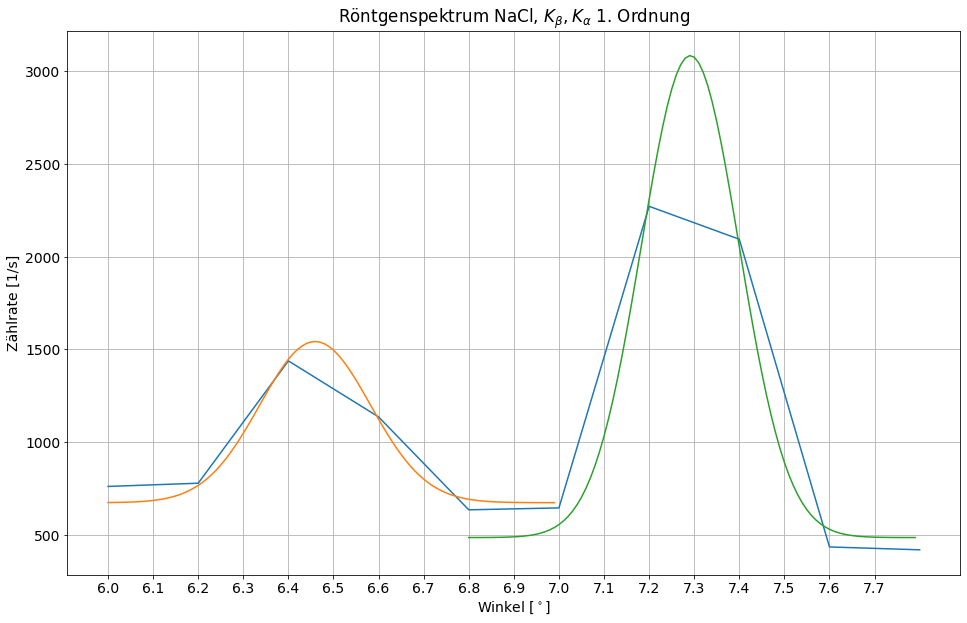
\includegraphics[width=.9\textwidth]{files/plots/nacl_k_1ord_fit.png}
  \caption{Fit an die K-Linien 1. Ordnung des Röntgengenspektrums, ausgemessen mit NaCl-Kristall.}
  \label{fig:nacl_k_1ord_fit}
\end{figure}


Für den Mittelwert dieser beiden Werte gilt also
\begin{align}
  d = (280.8 \pm 1.5)\si{\pico\meter}.
\end{align}

Dies ist der Netzebenenabstand von NaCl. Um die Gitterkonstante zu berechnen, verdoppeln wir diesen und erhalten
\begin{align}
  a = 2d = (561.6 \pm 2.9)\si{\pico\meter}.
\end{align}

Außerdem können wir nach Gleichung \eqref{eq:avogadro} anhand des Netzebenenabstands die Avogadrokonstante $N_A$ berechnen. Hierzu ziehen wir noch die Dichte von NaCl, $\rho = 2.164\si{\gram\per\centi\meter\cubed}$, und dessen Molekulargewicht, $M = 58.44\si{\gram}$, hinzu. Wir kommen damit auf einen Wert von
\begin{align}
  N_A = (6.10 \pm 0.10) \cdot 10^{23} \si{\per\mol}.
\end{align}